\chapter{Surface/Subsurface flow coupling -- H-Processes}
\label{sec:Coupling}
%
This chapter deals with the coupling of rivers and overland flow with the variably saturated zone and aquifers.
%
\section{Theory}
\label{sec:Coupling_theory}
%
For the coupling of flow processes on separate but adjacent domains exchange fluxes are calculated at common interfaces.
The exchange fluxes between overland and variably saturated flow read
%
\begin{eqnarray}
q_{of}^{sf} = k_{a'} \Lambda \left( h^{of} - h^{sf} \right),  \quad   \Lambda = \frac{K^c}{a'} ,\quad q_{sf}^{of} = - q_{of}^{sf}
\label{eqn:CoupFlux1}
\end{eqnarray}
%
where $h^{of}$ is the overland flow water head, $h^{sf}$ the matric head in the variably saturated zone, $\Lambda$ is the leakance, $a'$ the interface thickness, and the scaling factor $0\leq k_{a'}\leq 1$, given by
%
\begin{eqnarray}
k_{a'} &=& S^{2 (1-S)} \\
S &=&  \min\left( \max\left(\frac{H}{a'},0\right),1  \right),
\end{eqnarray}
%
where $H$ is the surface flow water depth, ensures that infiltration does not exceed the available water on the surface. For the coupling conductivity $K^c$ the saturated soil hydraulic conductivity is taken.

The exchange fluxes between overland and groundwater flow read
%
\begin{eqnarray}
q_{of}^{gf} = \Lambda \left( h^{of} - h^{gf} \right),\quad q_{gf}^{of} = - q_{of}^{gf}
\label{eqn:CoupFlux4}
\end{eqnarray}
%
where $h^{gf}$ is the groundwater flow head.
%
The exchange fluxes between river and groundwater flow read
%
\begin{eqnarray}
q_{of}^{gf} =  \frac{P}{B}  \Lambda \left( h^{of} - h^{sf} \right),\quad q_{gf}^{of} = - q_{of}^{gf}
\label{eqn:CoupFlux2}
\end{eqnarray}
%
where $P$ is the wetted perimeter and $B$ the channel width. For a channel with rectangular cross section $P = 2 H_a + B$.
Is the groundwater level below the river bed the exchange fluxes become
%
\begin{eqnarray}
q_{of}^{gf} =  \Lambda H,\quad q_{gf}^{of} = - q_{of}^{gf}.
\label{eqn:CoupFlux3}
\end{eqnarray}
%
%
\begin{figure} [htb!]
 \centering
% 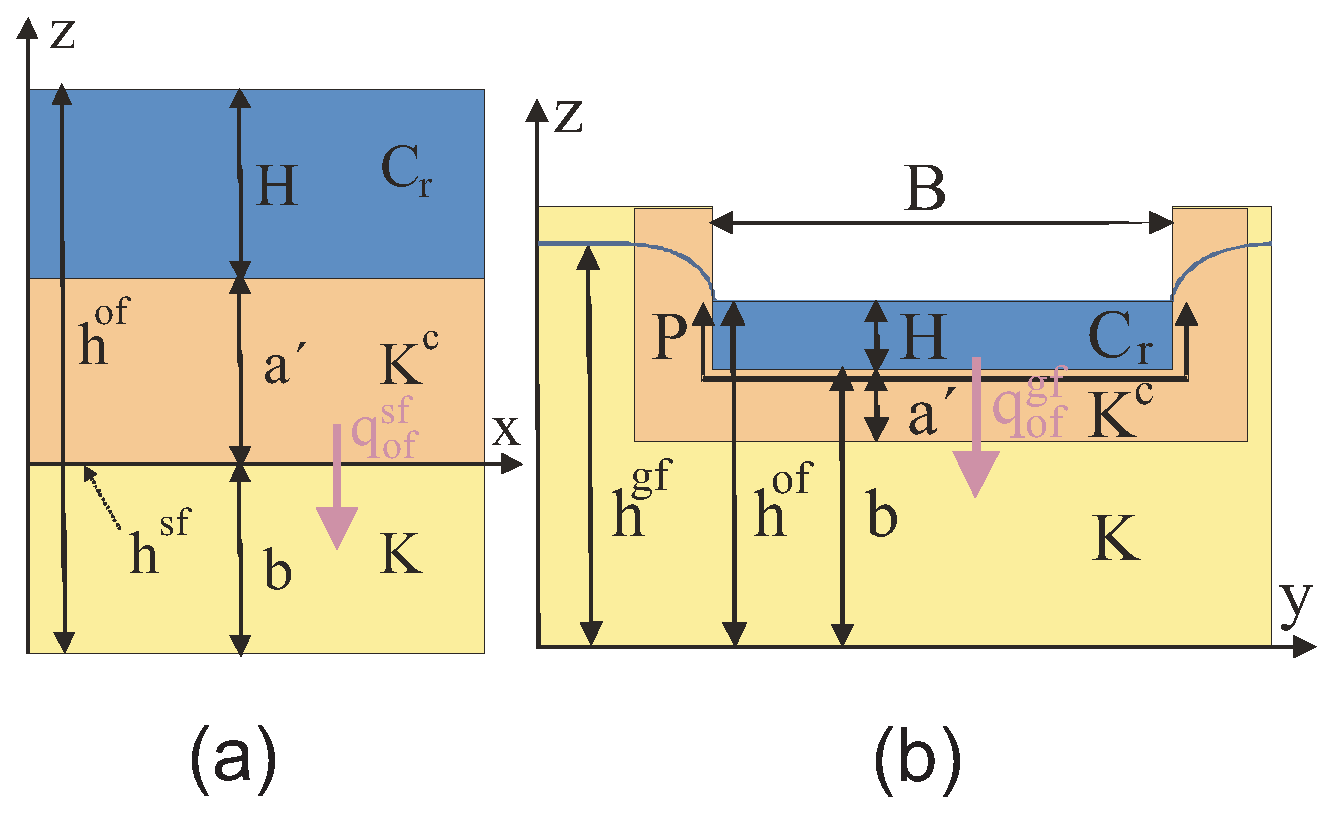
\includegraphics[width=0.75\columnwidth] {H_COUP/figures/exchangeFluxes.eps}
 \caption{Exchange fluxes between (a) overland and variably saturated flow $q_{of}^{sf}$, (b) river and aquifer flow $q_{of}^{gf}$, calculated with an interface (conductivity $K^c$) between the surface flow compartment (friction coefficient $C_r$) and variably zone/auifer compartment (conductivity $K$).}
 \label{coup:exchangeFluxes}
\end{figure}
%
%--------------------------------------------------------------------------------------------------------------------------
%
\section{Benchmarks examples}

\subsection{Horton flow}
\label{sec:CoupWoolhiser}
%
\subsubsection*{Problem definition}
%
This example is based on the experiments by Smith and Woolhiser, 1971 \cite{Smith:71} for initially drained conditions.
%
Infiltration excess overland (Hortonian) flow was generated by 15 minutes of artificial precipitation at a rate of 4.2 mm min$^{-1}$ on a soil flume
with a length of 12.2 m, a width of 5.1 cm, and a slope of 0.01. The experimental setup
is shown in Figure \ref{coup:woolhiserSetup} with the discretization meshes used in the simulations. Both overland and variably saturated flow are simulated one dimensionally with line elements.
%
\begin{figure} [htb!]
 \centering
 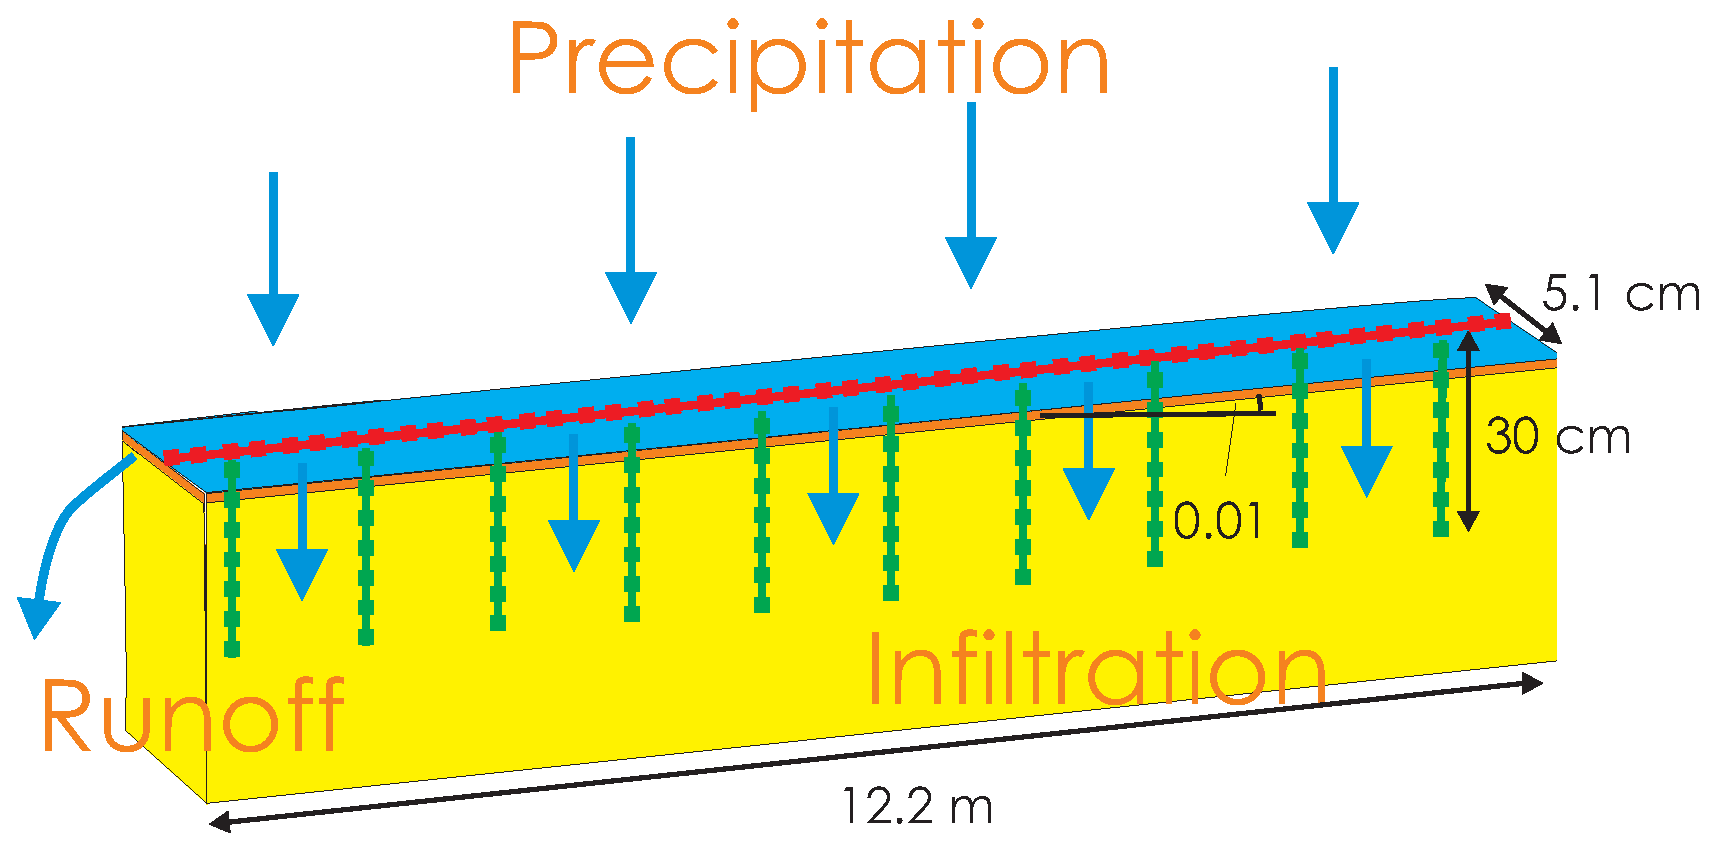
\includegraphics[width=0.75\columnwidth] {H_COUP/figures/woolhiserSetup.eps}
 \caption{Setup and discretization meshes in the Smith and Woolhiser, 1971 \cite{Smith:71} benchmark example.}
 \label{coup:woolhiserSetup}
\end{figure}
%
%%
\begin{table}[H]
 \centering
 \begin{tabular}{llll}
 \hline\hline\noalign{\smallskip}
 {\bf Items} & {\bf Symbol} & {\bf Setting} & {\bf Unit} \\ \hline \noalign{\smallskip}
 {\bf Fluid} & & & \\
 Kinematic viscosity            & $\nu$ & $177$ & mm$^2\,$min$^{-1}$  \\
 Density            & $\rho$ & $0.756$ & g$\,$mm$^{-3}$ \\ \hline \noalign{\smallskip}
{\bf Overland flow} & & & \\
 Surface friction  & $C$ & $80000$ & mm$^{-1}$min$^{-1} $ \\
 & $j$ & $1$ & $-$ \\
 & $l$ & $2$ & $-$ \\ \hline \noalign{\smallskip}
 {\bf Unsaturated flow} & & & \\
 Porosity             & $\phi$ & $0.42$ & $-$ \\
 Residual saturation & $S_r$ & $0.05$    &  $-$ \\
 Hydraulic conductivity & $K$ &  $1.7$  & mm$\, $min$^{-1}$\\
 Pore size   & $\alpha$ & $0.006$   &  mm$^{-1}$ \\
 Grain size distribution & $m$ & $0.75$  &  $-$ \\ \hline \noalign{\smallskip}
 {\bf Interface} & & & \\
 Conductivity  & $K^c$ & $1.7$ & mm$\,$min$^{-1}$\\
Thickness  & $a'$ & $1$ & mm \\
Immobile depth  & $a$ & $1$ & mm \\
\noalign{\smallskip}\hline\hline
 \end{tabular}
\centering
 \caption{Hydraulic parameters in the simulations of the laboratory experiment by Smith and Woolhiser, 1971 \cite{Smith:71}.}
 \label{us:WoolhiserSetting}
\end{table}
%
%
\subsubsection*{Initial and boundary conditions}
%
The overland flow compartment is initially dry ($H=1\times 10^{-6}$ m ) and initial soil saturation is $0.2$ uniformly.
A critical depth boundary condition assigned at the overland flow outlet.
At the residual boundaries no-flow is assigned
%
\begin{figure} [h!]
 \centering
\includegraphics[width=0.75\columnwidth] {H_COUP/figures/woolhiserResults.eps}
\caption{Simulated and measdured outflow hydrographs in the Smith and Woolhiser, 1971 \cite{Smith:71} benchmark example.}
 \label{coup:woolhiserResults}
\end{figure}
%
\subsubsection*{Material properties}
%
A uniform soil representation is chosen. Light oil was used as a fluid. Surface friction is described by
the laminar Ch\'{e}zy resistance to flow relationship. The soil-water-characteristic curves by
VanGenuchten are used.
Parameters are given in Table \ref{us:WoolhiserSetting}.
Wool\_little\_lines\_coup describes overland flow and soil flow one-dimensionally with line elements.
Wool\_little\_hex\_coup uses quadrants for overland flow which continue to three-dimensional soil flow hexahedra.
Time steps are $2s$.
The material and fluid properties used for the simulations are given in Tab.~\ref{us:WoolhiserSetting}.
Soil heterogeneity is neglected and the fluid parameters correspond to light oil. Surface friction is described by
the laminar Ch\'{e}zy resistance to flow relationship. The soil-water-characteristic curves by
VanGenuchten are used for the Richards soil flow description.
%

%
\subsubsection*{Results}
%
Runoff at the free-fall outlet is taken for comparison of experimental and simulation data (Figure \ref{coup:woolhiserResults}).
Time steps are 1 second. Line element sized for overland flow are $\Delta x = 12.2$ cm and for
flow in the variably saturated zone $\Delta x = 1$ mm.
%
\subsubsection*{Benchmark deposit}
%
\begin{tabular}{|l|l|l|}
  \hline
  Benchmark & Problem type & Path in benchmark deposit \\
  \hline
  \emph{Wool\_lines\_coup} & H & benchmarks\verb \COUPLED_FLOW\ \\
  \hline
\end{tabular}
%
%--------------------------------------------------------------------------------------------------------------------------
\subsection{Dunne flow}
\label{sec:CoupAbdul}
%
\subsubsection*{Problem definition}
%
This example is based on the experiments by Abdul and Gilham, 1984 \cite{Abdul:84} which 
were designed to examine the role of capillary fringe on runoff generation processes.
Precipitation was applied for 20 min on a soil flume with a length of 1.4 m, a width of 8 cm, and a slope of 0.12 (Figure \ref{coup:abdulflume}).
The initial groundwater level is set at the hight of the outlet such that immediately overland flow occurs. 
In the simulations the flume part
above the initial groundwater level is simulated with Richards equation and below with Darcy groundwater equation.
%
%
\begin{figure} [htb!]
 \centering
 \includegraphics[width=0.75\columnwidth] {H_COUP/figures/abdulflume.eps}
 \caption{Setup of the Abdul and Gilham, 1984 \cite{Abdul:84} benchmark example.}
 \label{coup:abdulflume}
\end{figure}
%
%%
\begin{table}[H]
 \centering
 \begin{tabular}{llll}
 \hline\hline\noalign{\smallskip}
 {\bf Items} & {\bf Symbol} & {\bf Setting} & {\bf Unit} \\ \hline \noalign{\smallskip}
{\bf Overland flow} & & & \\
 Surface friction  & $C$ & $5.39$ & m$^{1/3}$s$^{-1} $ \\
Immobile depth  & $a$ & $0.5$ & mm \\ \hline \noalign{\smallskip}
 {\bf Variably saturated flow} & & & \\
 Porosity             & $\phi$ & $0.34$ & $-$ \\
 Residual saturation & $S_r$ & $0.0$    &  $-$ \\
 Hydraulic conductivity & $K$ &  $5\times 10^{-5}$  & m$\, $s$^{-1}$\\
 Pore size   & $\alpha$ & $2.4$   &  m$^{-1}$ \\
 Grain size distribution & $m$ & $0.8$  &  $-$ \\ \hline \noalign{\smallskip}
 {\bf Groundwater flow} & & & \\
 Porosity             & $\phi$ & $0.34$ & $-$ \\
 Specific storage            & $S$ & $0.0$ & $-$ \\ \hline \noalign{\smallskip}
 {\bf Overland/soil Interface} & & & \\
 Conductivity  & $K^c$ & $5\times 10^{-5}$  & m$\, $s$^{-1}$\\
Thickness  & $a'$ & $0.5$ & mm \\
{\bf Soil/aquifer Interface} & & & \\
Leakance  & $\Lambda$ & $5\times 10^{-4}$  & s$^{-1}$\\
\noalign{\smallskip}\hline\hline
 \end{tabular}
\centering
 \caption{Hydraulic parameters in the simulations of the laboratory experiment by Abdul and Gilham, 1984 \cite{Abdul:84}.}
 \label{us:WoolhiserSetting}
\end{table}
%
\subsubsection*{Initial and boundary conditions}
%

%
\subsubsection*{Material properties}
%

%

%
\subsubsection*{Results}
%
Measured and simulated outflow are compared in Fig.~\ref{coup:abdul_results}.

\begin{figure} [htb!]
 \centering
\includegraphics[width=0.75\columnwidth] {H_COUP/figures/abdul_results.eps}
\caption{Simulated and measured outflow hydrographs in the Abdul and Gilham, 1984 \cite{Abdul:84} benchmark example.}
 \label{coup:abdul_results}
\end{figure}
%
\subsubsection*{Benchmark deposit}
%
\begin{tabular}{|l|l|l|}
  \hline
  Benchmark & Problem type & Path in benchmark deposit \\
  \hline
  \emph{abdul\_lab} & H & benchmarks\verb \COUPLED_FLOW\ \\
  \hline
\end{tabular}
%
%
%
\subsection{Aquifer recharge from channel}
%
\subsubsection*{Problem definition}
%
This example deals with a confined aquifer with inflow by a rectangular channel (Figure \ref{coup:river_setup}). An analytical solution is given by Glover, 1978 \cite{Glover:78}.
%
\begin{figure} [htb!]
 \centering
 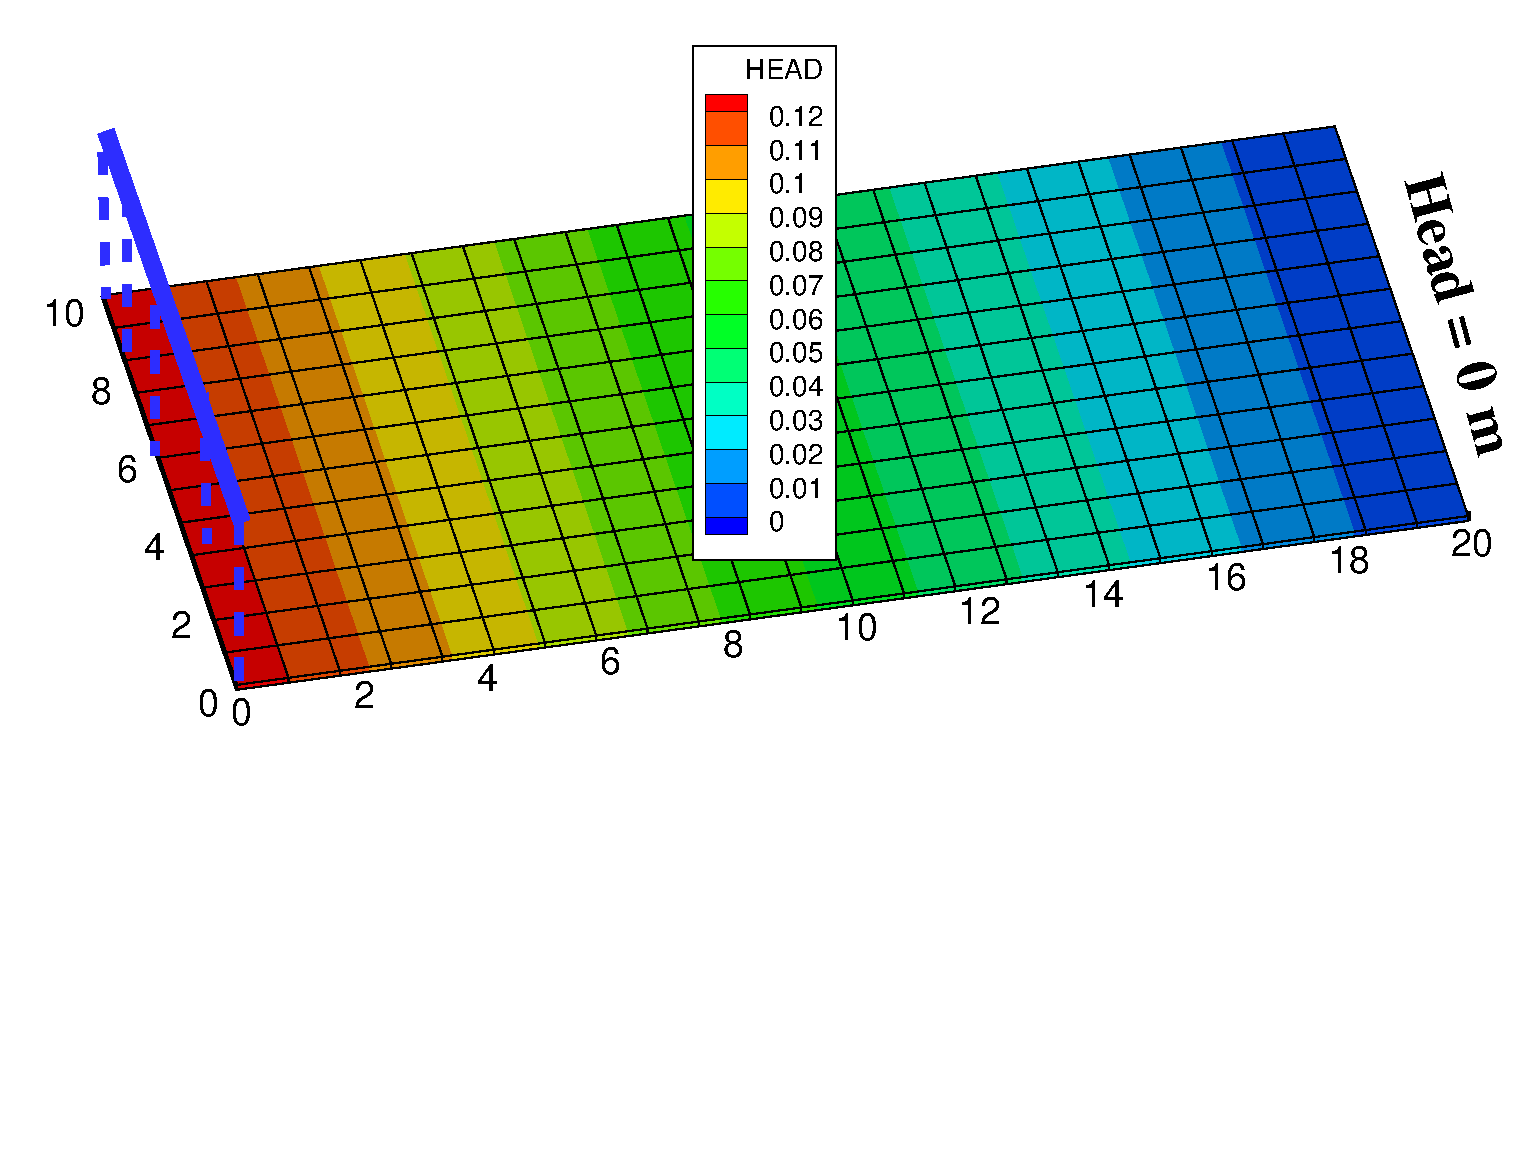
\includegraphics[width=0.75\columnwidth] {H_COUP/figures/river_setup.eps}
 \caption{Setup of the Glover, 1978 \cite{Glover:78} benchmark example.}
 \label{coup:river_setup}
\end{figure}
%

\subsubsection*{Initial and boundary conditions}
%
Channel initial and boundary conditions are $3m$ for water depth. Initial groundwater head is $0m$. The head at the boundary opposite of the channel is $0$. At the remaining boundaries no-flow is imposed.
%
\begin{figure} [htb!]
 \centering
\includegraphics[width=0.75\columnwidth] {H_COUP/figures/river_results.eps}
\caption{Comparison of Simulated groundwater depths below the river bed with the analytical solution by Glover, 1978 \cite{Glover:78}.}
 \label{coup:river_results}
\end{figure}
%
\subsubsection*{Material properties}
%
The domain is discretized with $24\times 12$ quadrants and the time step size is $60s$.
Simulation parameters are given in Tab.~\ref{Coup_ChannelPercolation}.
%
\begin{table}[H]
 \centering
 \caption{Parameters for aquifer recharge example}
 \centering \label{Coup_ChannelPercolation}
 \begin{tabular}{llll}
 \hline\hline\noalign{\smallskip}
 {\bf Parameter} & {\bf Symbol} & {\bf Setting} & {\bf Unit} \\ \hline
 Friction coefficient & $C$ & $333$ & $ms$ \\
 Corresponding Manning coefficient & $n$ & $3\times 10^{-3}$ & $1/ms$ \\
 Channel width & $B$ & $14$ & $m$ \\
 Leakance & $3.33\times 10^{-6}$ & $1/s$ & \\
 Rill depth/ Interface layer thickness & $a$ & $0$ & $m$ \\
 Surface structure parameter & $\epsilon$ & $0$ & $m$  \\
 Specific yield  & $S_y$ & $0.2$ & $1/m$ \\
 Permeability  & $k$ & $1\times 10^{-3}$ & $m^2$\\
 Aquifer thickness & $L$ & $25$ & $m$ \\ \hline
\noalign{\smallskip}\hline\hline
 \end{tabular}
\end{table}
%
\subsubsection*{Results}
%
Comparison of simulation results and analytical solution is shown in Fig.~\ref{coup:river_results}.
%
\subsubsection*{Benchmark deposit}
%
\begin{tabular}{|l|l|l|}
  \hline
  Benchmark & Problem type & Path in benchmark deposit \\
  \hline
  \emph{riv1\_quad\_coup} & H & benchmarks\verb \COUPLED_FLOW\ \\
 \hline
\end{tabular}
%
%--------------------------------------------------------------------------------------------------------------------------
%
\subsection{Flood at channel junction}
%
\subsubsection*{Problem definition}
%
Two uniform rectangular channels confluence symmetrically and form a larger rectangular channel which continues uniformly. The aquifer is
unconfined, flat, homogeneous, and has a size of $10000m\times 4000m$ (Figure \ref{coup:riverJunction_setup}).
A flood waves starts propagating at both upstream inlets and merge at the junction. Manning's roughness coefficient is constant throughout as well as the slope of about $0.0001$.
The total time is $5$ days and comprises a part of the rising limb of the flood.
Two scenarios are considered by varying the aquifer initial conditions such that flow occurs from the channels to the aquifer or vice versa. The total time is $30$ days and comprises the rising and falling limb of the flood.
These examples were proposed by \cite{Gunduz:05}. Benchmarking is based on code comparison.
%
\begin{figure} [htb!]
 \centering
 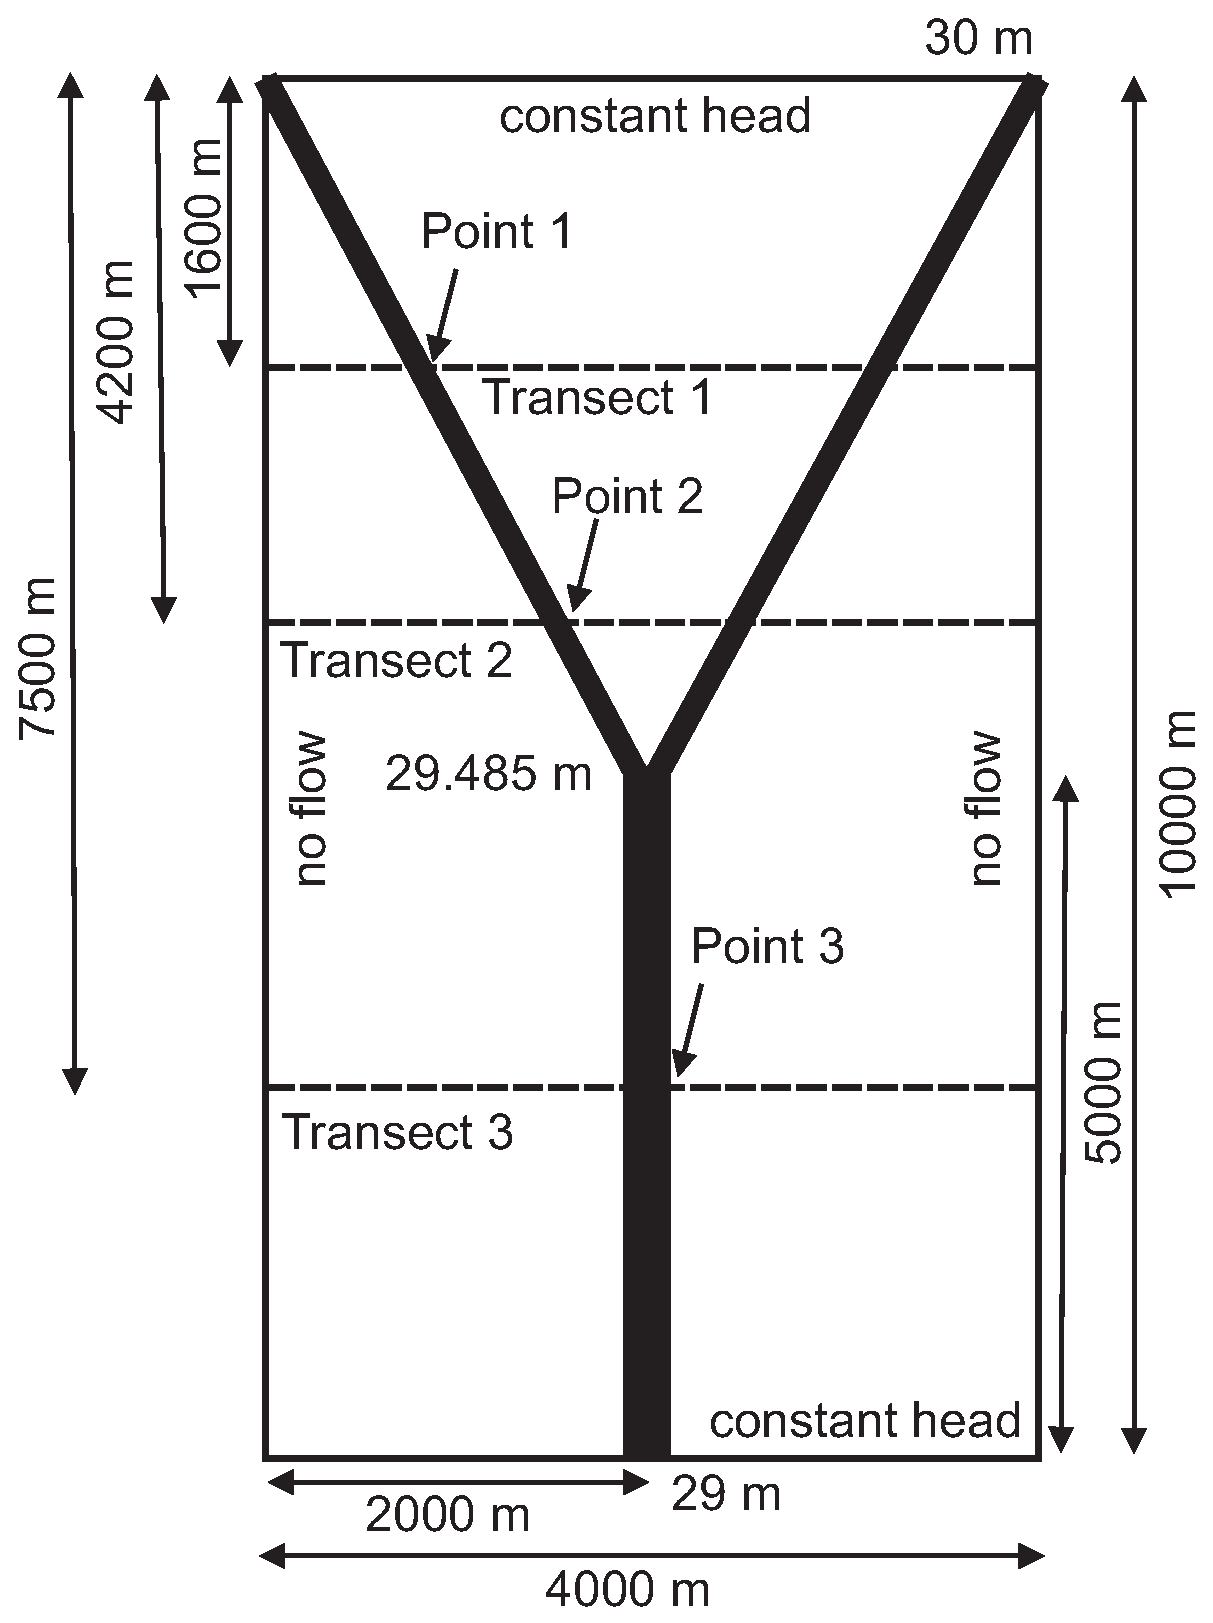
\includegraphics[width=0.75\columnwidth] {H_COUP/figures/riverJunction_setup.eps}
 \caption{Setup of the Gunduz and Aral, 2005 \cite{Gunduz:05} benchmark example.}
 \label{coup:riverJunction_setup}
\end{figure}
%
%
\subsubsection*{Initial and boundary conditions}
%
Initial water depth in the rivers is $4.5m$ and the aquifer is set at $z = 0$.  The initial head for the aquifer is $h =32$ m for scenario I and $h=35$ m for scenario II.
At the  aquifer boundaries constant head and no-flow conditions are imposed (Figure \ref{coup:riverJunction_setup}). At the river inlets the inflow rises linearly from $100 m^3/s$ to $350 m^3/s$
between $t= 3$ and $t=10$ days and declines again linearly to the initial value between $t=11$ and $t= 17$ days. At the channel outlet a normal depth boundary condition is assigned.
%
\subsubsection*{Material properties}
The simulation parameters for the channels and aquifer are given in Tab.~\ref{Coup_ChannelPercolation}.
%
\begin{table}[H]
 \centering
 \caption{Parameters for channel junction examples}
 \centering \label{Coup_ChannelPercolation}
 \begin{tabular}{llll}
 \hline\hline\noalign{\smallskip}
 {\bf Items} & {\bf Symbol} & {\bf Setting} & {\bf Unit} \\ \hline
 Friction coefficient & $C$ & $40$ & $ms$ \\
 Corresponding Manning coefficient & $n$ & $0.025$ & $1/ms$ \\
 Width of upstream channels & $B$ & $30$ & $m$ \\
 Width of downstream channel & $B$ & $45$ & $m$ \\
 Leakance & $\Lambda $& $3.33\times 10^{-6}$ & $1/s$  \\
 Rill depth/ Interface layer thickness & $a$ & $0$ & $m$ \\
 Surface structure parameter & $\epsilon$ & $0$ & $m$  \\
 Specific yield & $S_y$ & $0.2$ & $1/m$ \\
 Permeability  & $k$ & $1\times 10^{-9}$ & $m^2$\\
\noalign{\smallskip}\hline\hline
 \end{tabular}
\end{table}
%
\subsubsection*{Results}
%
Figs.~\ref{coup:riverJunction_scenarioI_points}-\ref{coup:riverJunction_scenarioI_transectII} show groundwater heads and river stages at Points 1-3 and groundwater heads at transect I for both
scanario I and II.
%
\begin{figure} [htb!]
 \centering
 \includegraphics[width=0.75\columnwidth] {H_COUP/figures/riverJunction_scenarioI_points.eps}
 \caption{Groundwater heads and river stages of the Gunduz and Aral, 2005 \cite{Gunduz:05} benchmark example for scenario I.}
 \label{coup:riverJunction_scenarioI_points}
\end{figure}
%
\begin{figure} [htb!]
 \centering
 \includegraphics[width=0.75\columnwidth] {H_COUP/figures/riverJunction_scenarioI_transectI.eps}
 \caption{Groundwater heads at transect I of the Gunduz and Aral, 2005 \cite{Gunduz:05} benchmark example for scenario I.}
 \label{coup:riverJunction_scenarioI_transectI}
\end{figure}
%
\begin{figure} [htb!]
 \centering
 \includegraphics[width=0.75\columnwidth] {H_COUP/figures/riverJunction_scenarioII_points.eps}
 \caption{Groundwater heads and river stages of the Gunduz and Aral, 2005 \cite{Gunduz:05} benchmark example for scenario II.}
 \label{coup:riverJunction_scenarioII_points}
\end{figure}
%
\begin{figure} [htb!]
 \centering
 \includegraphics[width=0.75\columnwidth] {H_COUP/figures/riverJunction_scenarioII_transectI.eps}
 \caption{Groundwater heads at transect I of the Gunduz and Aral, 2005 \cite{Gunduz:05} benchmark example for scenario II.}
 \label{coup:riverJunction_scenarioI_transectII}
\end{figure}
%
\subsubsection*{Benchmark deposit}
\begin{tabular}{|l|l|l|}
  \hline
  Benchmark & Problem type & Path in benchmark deposit \\
  \hline
  \emph{biFork1\_coup} & H & benchmarks\verb \COUPLED_FLOW\ \\
  \emph{biFork2\_coup} & H & benchmarks\verb \COUPLED_FLOW\ \\
 \hline
\end{tabular}


